\documentclass{article}
\usepackage{shorttoc}
\usepackage[utf8]{inputenc}
\usepackage[T1]{fontenc}
\usepackage{fancyhdr}
\usepackage{lastpage}
\usepackage{graphicx}
\usepackage[left=2cm,right=2cm,top=3cm,bottom=2cm]{geometry}
\title{Programmation Parralèlle - Cours (1)}
\author{David GUERROUDJ}
\date{\today}
 
\rfoot{Page \thepage \hspace{1pt} sur \pageref{LastPage}}
 
\begin{document}

\maketitle % Page de garde.

\tableofcontents % Table des matières
\vfill\eject

\section{Qu'est-ce qu'un thread ?}
C'est un objet qui va effectuer une tache. Il existe deux moyens de créer un thread:
\begin{enumerate}
\item  en créant une classe qui hérite de Thread :
Elle doit alors implémenther une méthode run qui permet de lancer l'objet.
\item En créant une classe qui implémente l'inferface Runnable : L'héritage multiple étant interdit, cela permet d'hériter d'une autre classe.
\end{enumerate}

\section{Fonctions importantes}
\begin{enumerate}
\item Sleep()
\item Join() $ \rightarrow $ très importante !
\item wait()
\end{enumerate}

\section{Différents états possible d'un thread}
\begin{enumerate}
\item Execute son code cible ( il a un accès à l'un des processeurs )
\item attend l'accès à un processeur ( mais pourrait s'exécuter )
\item attend un événement particulier ( pour etre autorisé à commencer, ou poursuvre son exécution)
\end{enumerate}
Un thread peut avoir plusieurs états :
\begin{enumerate}
\item{1} création : le thread vient d'être créé, mais il n'a pas encore été exécuté,
\item{2} exécutable : le thread est candidat à l'exécution, il attend que le système lui alloue le processeur pendant une certaine durée, appelée quantum de temps,
\item{3} en cours d'exécution : le thread est en cours d'exécution par le processeur (sur un système monoprocesseur, un seul thread peut se trouver dans cet état),
\item{4} bloqué : le thread a provoqué une opération bloquante ou s'est "endormi" volontairement pour une certaine durée,
\item{5} détruit : le thread a fini son exécution ou a été arrêté par un autre thread.
\end{enumerate}
Voici un schéma montrant l'ordre de passage des différents états :\\
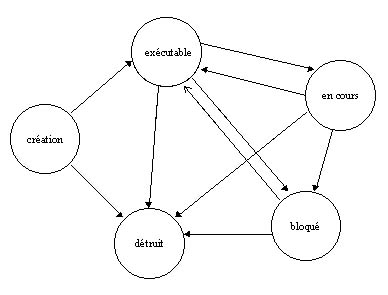
\includegraphics{images/1.jpg}
\section{Volatile}
Si une variable est partagé par plusieurs threads, doit etre déclarée volatille, sinon il y a risque qu'elle ne soit pas affectées (vue entre les threads).

\section{Ce qu'il faut retenir}
\begin{enumerate}
\item Il ne faut pas utiliser yield pour utiliser un programme correcte. Yield fait qu'un programme est plus performant.
\item L'utilisation de volatile.
\item L'utilisation de verrous, mieux faut utiliser synchonized.
\item L'utilisation des méthodes : wait(), sleep(), join().
\item La méthode wait necessite l'utilisation des verrous à l'aide de synchronized.
\end{enumerate}
\end{document}	
	